% no answer key
% \documentclass[letterpaper]{exam}

% answer key
\documentclass[letterpaper, landscape]{exam}
\usepackage{2in1, lscape} 
\printanswers{}

\usepackage{units} 
\usepackage{xfrac} 
\usepackage[fleqn]{amsmath}
\usepackage{cancel}
\usepackage{float}
\usepackage{mdwlist}
\usepackage{booktabs}
\usepackage{cancel}
\usepackage{polynom}
\usepackage{caption}
\usepackage{fullpage}
\usepackage{comment}
\usepackage{enumerate}
\usepackage{graphicx}

\newcommand{\degree}{\ensuremath{^\circ}} 
\everymath{\displaystyle}

\title{Statistics \\ Homework Two}
\author{}
\date{\today}

\begin{document}

  \maketitle

  \section{Homework}

  \begin{itemize*}
    \item read Chapter 2 
    \item answer the questions in ``Check Your Skills'' and check the answers
      in the back of the book
    \item hand in exercises 25--27, 29--30, 37--39, 41--43, 45, 50--51
  \end{itemize*}

  \ifprintanswers{}
    \section{Solutions}

    \begin{description}
      \item[25] The larger number is the mean because the mean is dragged upward by a few
        people who make hundreds of thousands of dollars.

      \item[26] 
        For the people who are still working (21--54), there are a lot of young people with
        almost no retirement money and a few older people with large retirement accounts.
        This makes the distribution right-skewed and the mean is larger than the median.

        For the people who are mostly retired (55 or older), almost everyone has some
        retirement money saved, and there are only a few people with no retirement money.
        This makes the distribution left-skewed and the mean is smaller than the median.

      \item[27] 
        \begin{align*}
          Q_1           & = 196.5 \\
          \text{median} & = 393 \\
          Q_3           & = 589.5 \\
        \end{align*}

      \item[29]
        \begin{figure}[H]
          \centering
          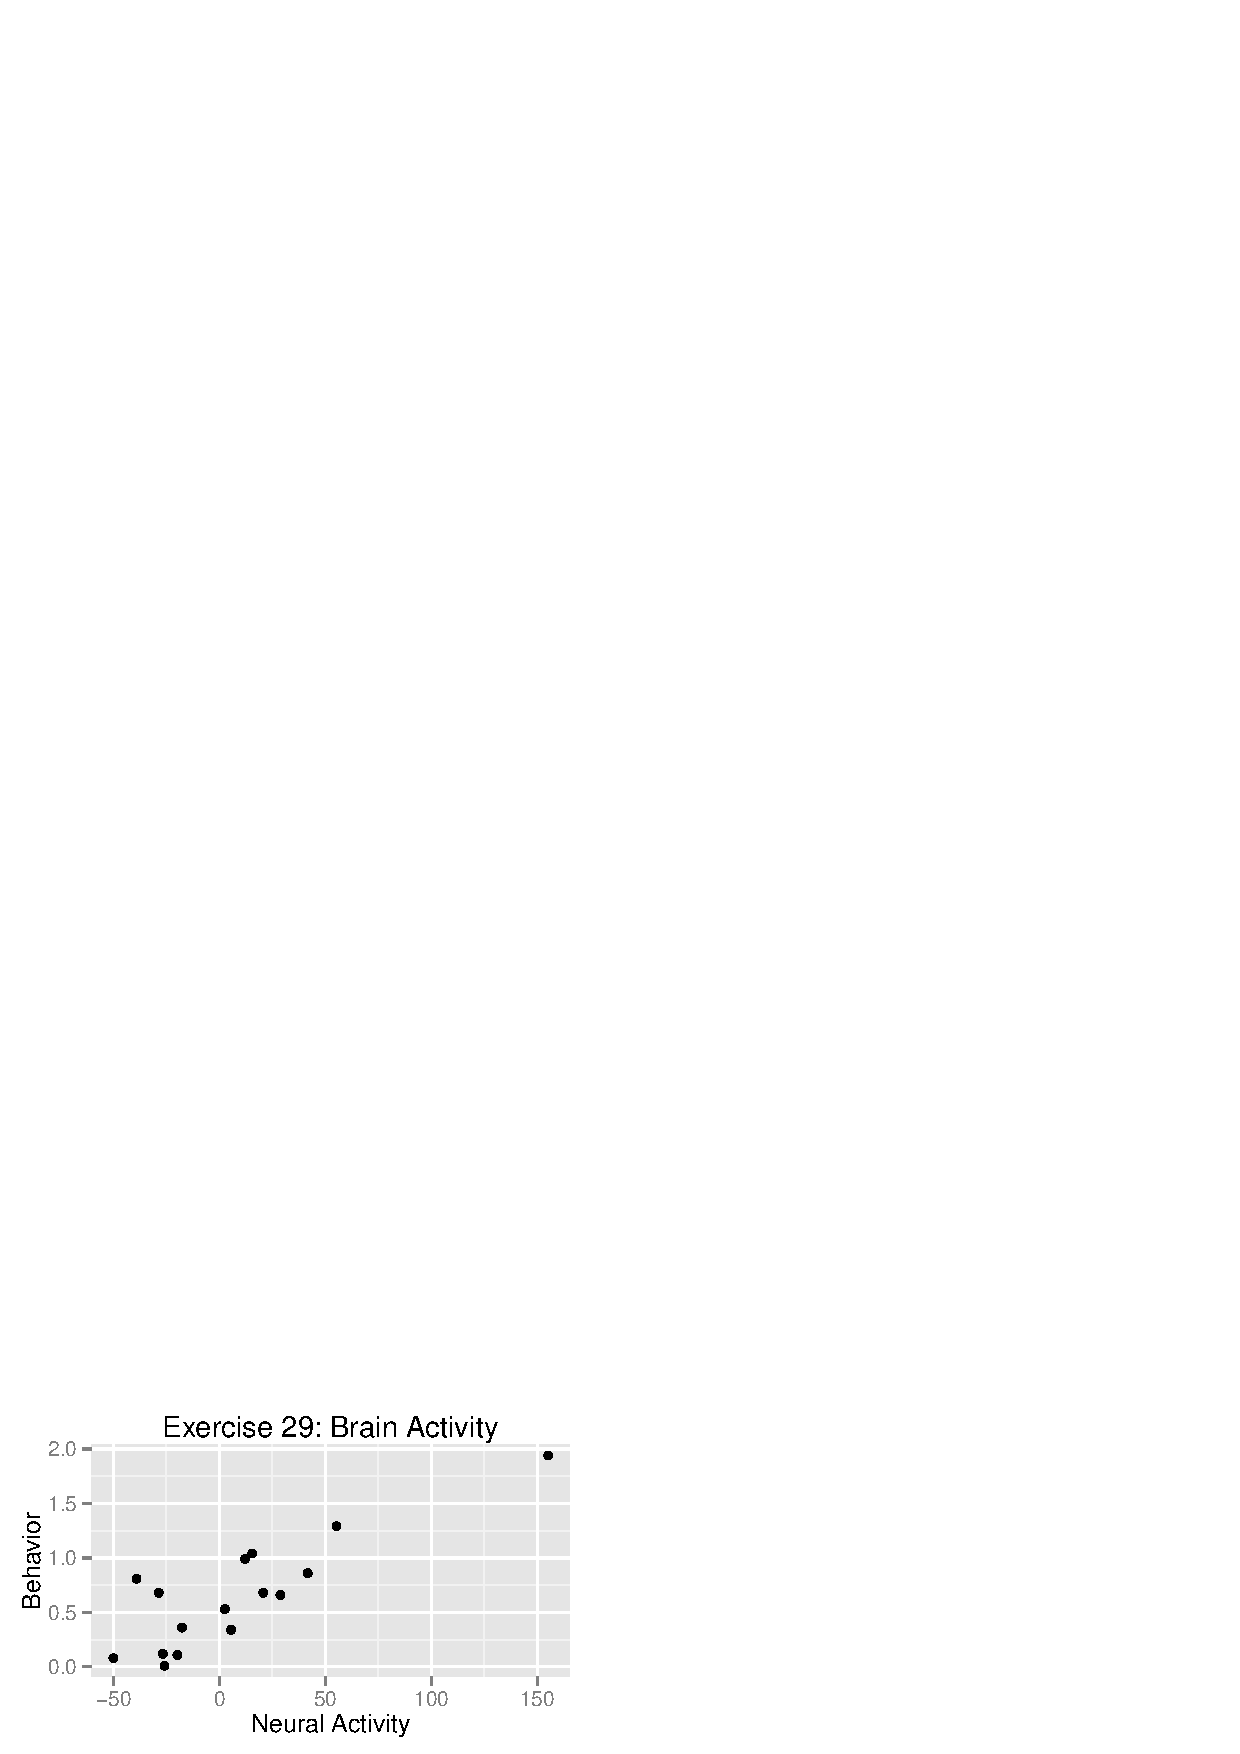
\includegraphics{figures/ex29.pdf}
          \caption{Exercise 29}
        \end{figure}

        \begin{table}[H]
          \centering
          \begin{tabular}{rlrrrrrr}
            \toprule
              & Variety & Min.  & 1st Qu. & Median & Mean  & 3rd Qu. & Max. \\
            \midrule
            1 & Bihai   & 46.34 & 46.73   & 47.12  & 47.60 & 48.20   & 50.26 \\
            2 & Red     & 37.40 & 38.08   & 39.16  & 39.71 & 41.58   & 43.09 \\
            3 & Yellow  & 34.57 & 35.56   & 36.11  & 36.18 & 36.80   & 38.13 \\
            \bottomrule
          \end{tabular}
        \end{table}

        The summary doesn't show the shape that the histogram does.

      \newpage

      \item[30]
        If you add up all the bars, you find that there are 77 girls.  
        
        \begin{itemize*}
          \item The median would be girl number 39, which would be in the 2 servings bar.  
          \item The first quartile would be girl 19 which is in the 1 serving bar.
          \item The third quartile would be girl 58 which is in the 4 servings bar.  
        \end{itemize*}

        \begin{align*}
          Q_1           & = 1 \\
          \text{median} & = 2 \\
          Q_3           & = 4 \\
        \end{align*}

      \item[37]
        The average of the individual state averages is only 8.4\%.

        The big states have more people so they have a greater affect on the
        national average than the small states.  Since the big states all have
        high percentages of foreign-born people, the national average is higher
        than the average of all the states individually.

      \item[38]
        For the median to be zero, half the households must have no credit card
        debt.  There are probably quite a few households that have no credit
        cards at all, so they don't have any credit card debt.  And even if you
        just look at credit card holders, there are probably quite a few people
        who pay their credit cards every month and don't have any debt.

      \item[39]
        \begin{enumerate}
          \item You can get a standard deviation of 0 by choosing the same number four times.

          \item You get the maximum standard deviation by choosing two 0s and two 10s.

          \item Any number works for part a.  There is only one correct answer for part b.
        \end{enumerate}

      \item[41]
        For the mean to be 7, the five numbers must add up to 35.  For the
        median to be 10, the third number in the sequence must be 10.

        Since the mean needs to be less than the median, it makes sense to use
        as small numbers as possible.  If the last three numbers are all 10s,
        the middle number will be 10.  Then the first two numbers need to add
        to 5 to get the total to 35.

        A few sets of numbers that work with this approach are: 
        
        \{1, 4, 10, 10, 10 \} and \{2, 3, 10, 10, 10\}.

        Once you see this, you can make other choices for the last two numbers,
        as long as you don't make them so large that you can't get the mean
        down to 7.  

      \item[42]
        For the mean to be larger than the third quartile, you just need one
        really large number.  Here is a set that works: 
        
        \{1, 2, 3, 4, 5, 100 \}.  
        
        The third quartile is 5 and the mean is 19.17.

      \item[43]

        The summary for the owner might be:
        \begin{itemize*}
          \item half the players make \$2.8M or less
          % \item Manny Ramirez is the highest paid player on the team at \$1.7M.
          %   Curt Schilling and David Ortiz are next at \$1.3M.
          \item The top three players (Ramirez, Schilling, and Ortiz) account
            for 35\% of the payroll
          % \item Jacoby Ellsbury, Manny Delcarmen and Dustin Pedroia are the
          %   lowest paid players at \$380,000.
          \item The mean salary is \$5M.
          \item The total payroll is \$127M
        \end{itemize*}

        \begin{table}[H]
          \centering
          \begin{tabular}{rr}
            \toprule
            Min.    & \$380,000 \\
            1st Qu. & \$424,500 \\
            Median  & \$2,800,000 \\
            Mean    & \$5,066,000 \\
            3rd Qu. & \$8,625,000 \\
            Max.    & \$17,020,000 \\
            \bottomrule
          \end{tabular}
          \caption{Exercise 43}
        \end{table}
        \begin{figure}[H]
          \centering
          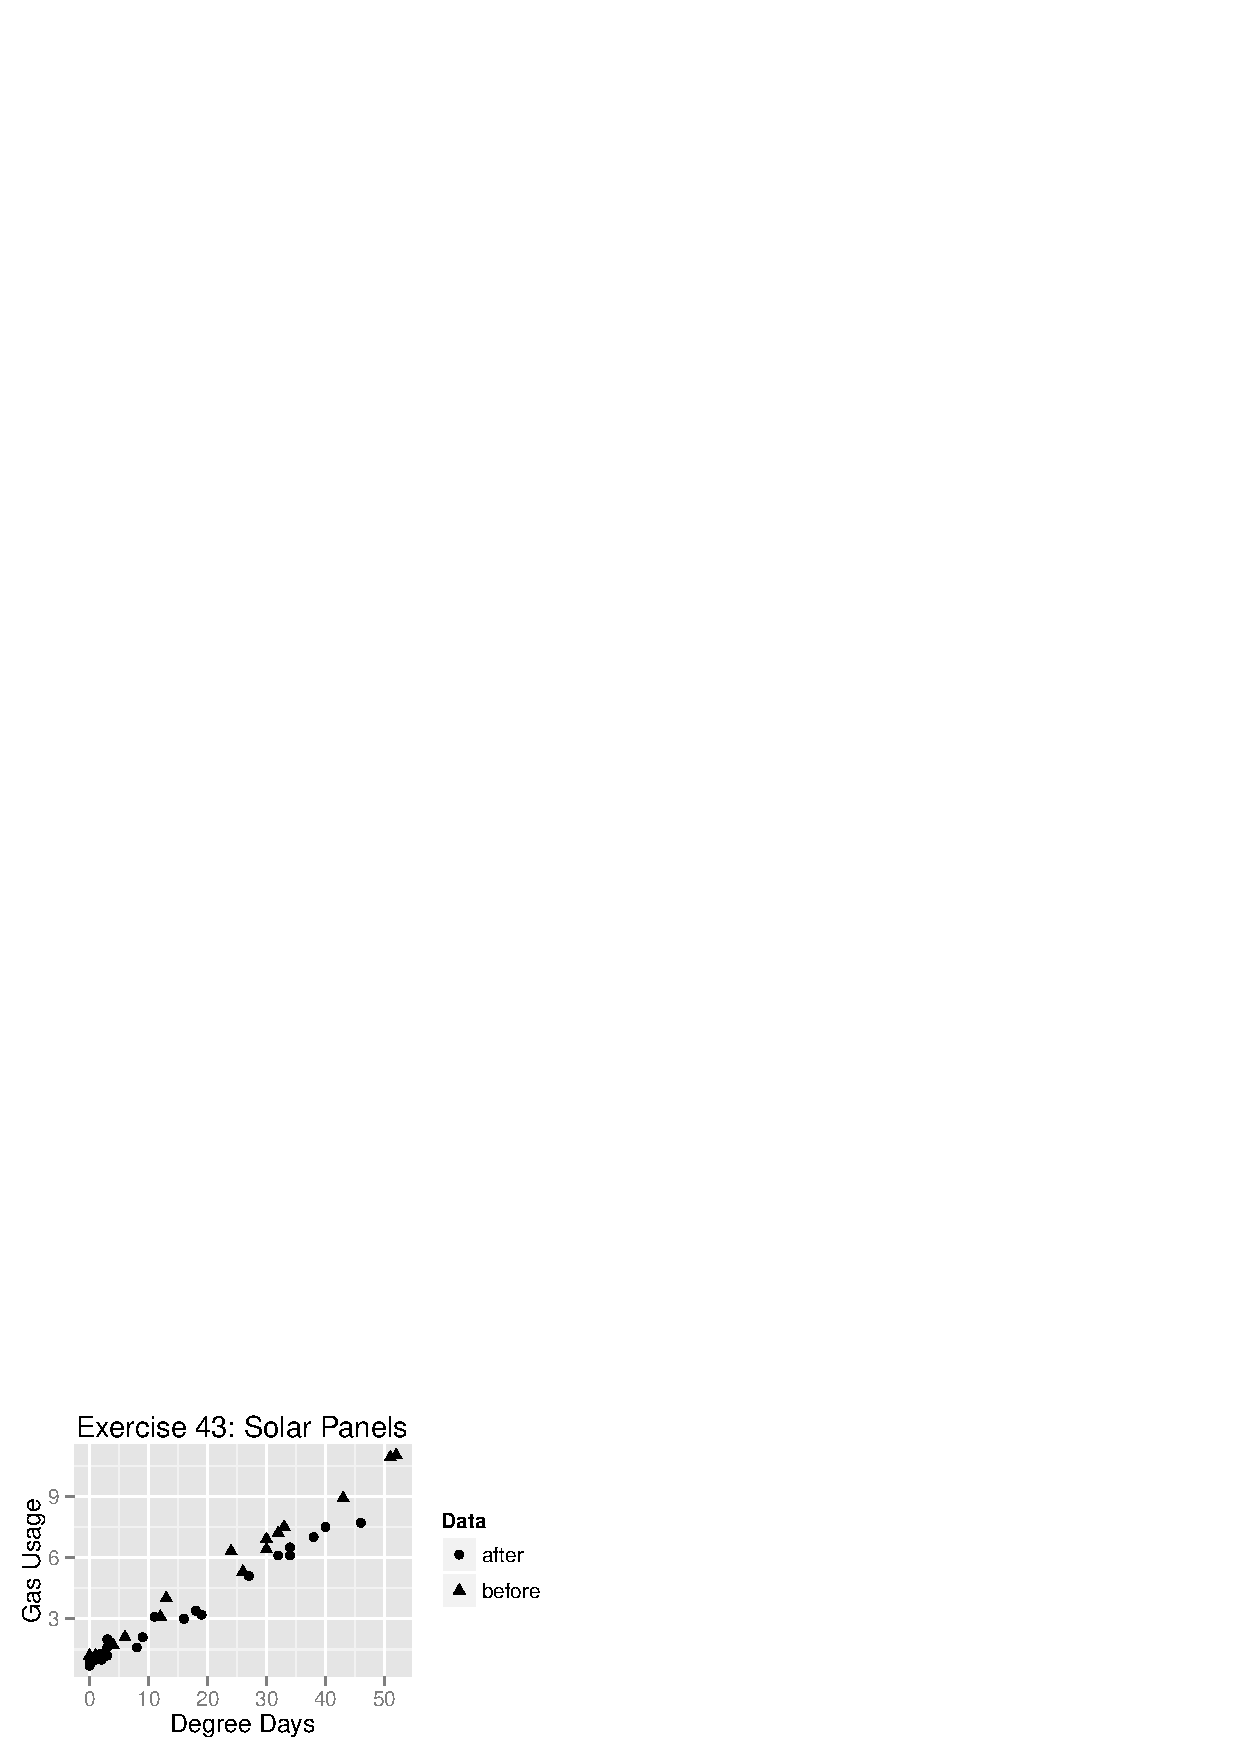
\includegraphics{figures/ex43.pdf}
          \caption{Exercise 43 Histogram}
        \end{figure}

      \item[45]
        Either odor makes people spend more money but lavender is
        more effective than lemon.

        \begin{table}[H]
          \centering
          \begin{tabular}{rlrr}
            \toprule
              & Odor     & Median & Mean \\
            \midrule
            1 & Lavender & 22     & 21 \\
            2 & Lemon    & 18     & 18 \\
            3 & No Odor  & 17     & 18 \\
            \bottomrule
          \end{tabular}
          \caption{Exercise 45}
        \end{table}

        \begin{figure}[H]
          \centering
          \includegraphics{figures/ex45.pdf}
          \caption{Exercise 45 Box Plot}
        \end{figure}

        \begin{figure}[H]
          \centering
          \includegraphics{figures/ex45_histogram.pdf}
          \caption{Exercise 45 Histogram}
        \end{figure}


      \item[50]
        \begin{table}[ht]
          \centering
          \begin{tabular}{lr}
            \toprule
            Min.    & 0.10 \\
            1st Qu. & 0.97 \\
            Median  & 3.30 \\
            Mean    & 4.73 \\
            3rd Qu. & 7.20 \\
            Max.    & 19.60 \\
            \bottomrule
          \end{tabular}
          \caption{Exercise 50}
        \end{table}

        Since the mean is larger than the median, the distribution is right-skewed.
        According to the rule:
        \[
          outlier = 7.2 + 1.5 \times (7.2 - 0.97) \approx 16.5 \\
        \]

        US, Canada, and Australia are outliers according to the rule.  This
        makes sense when you look at the histogram or stem plot.

        \begin{figure}[H]
          \centering
          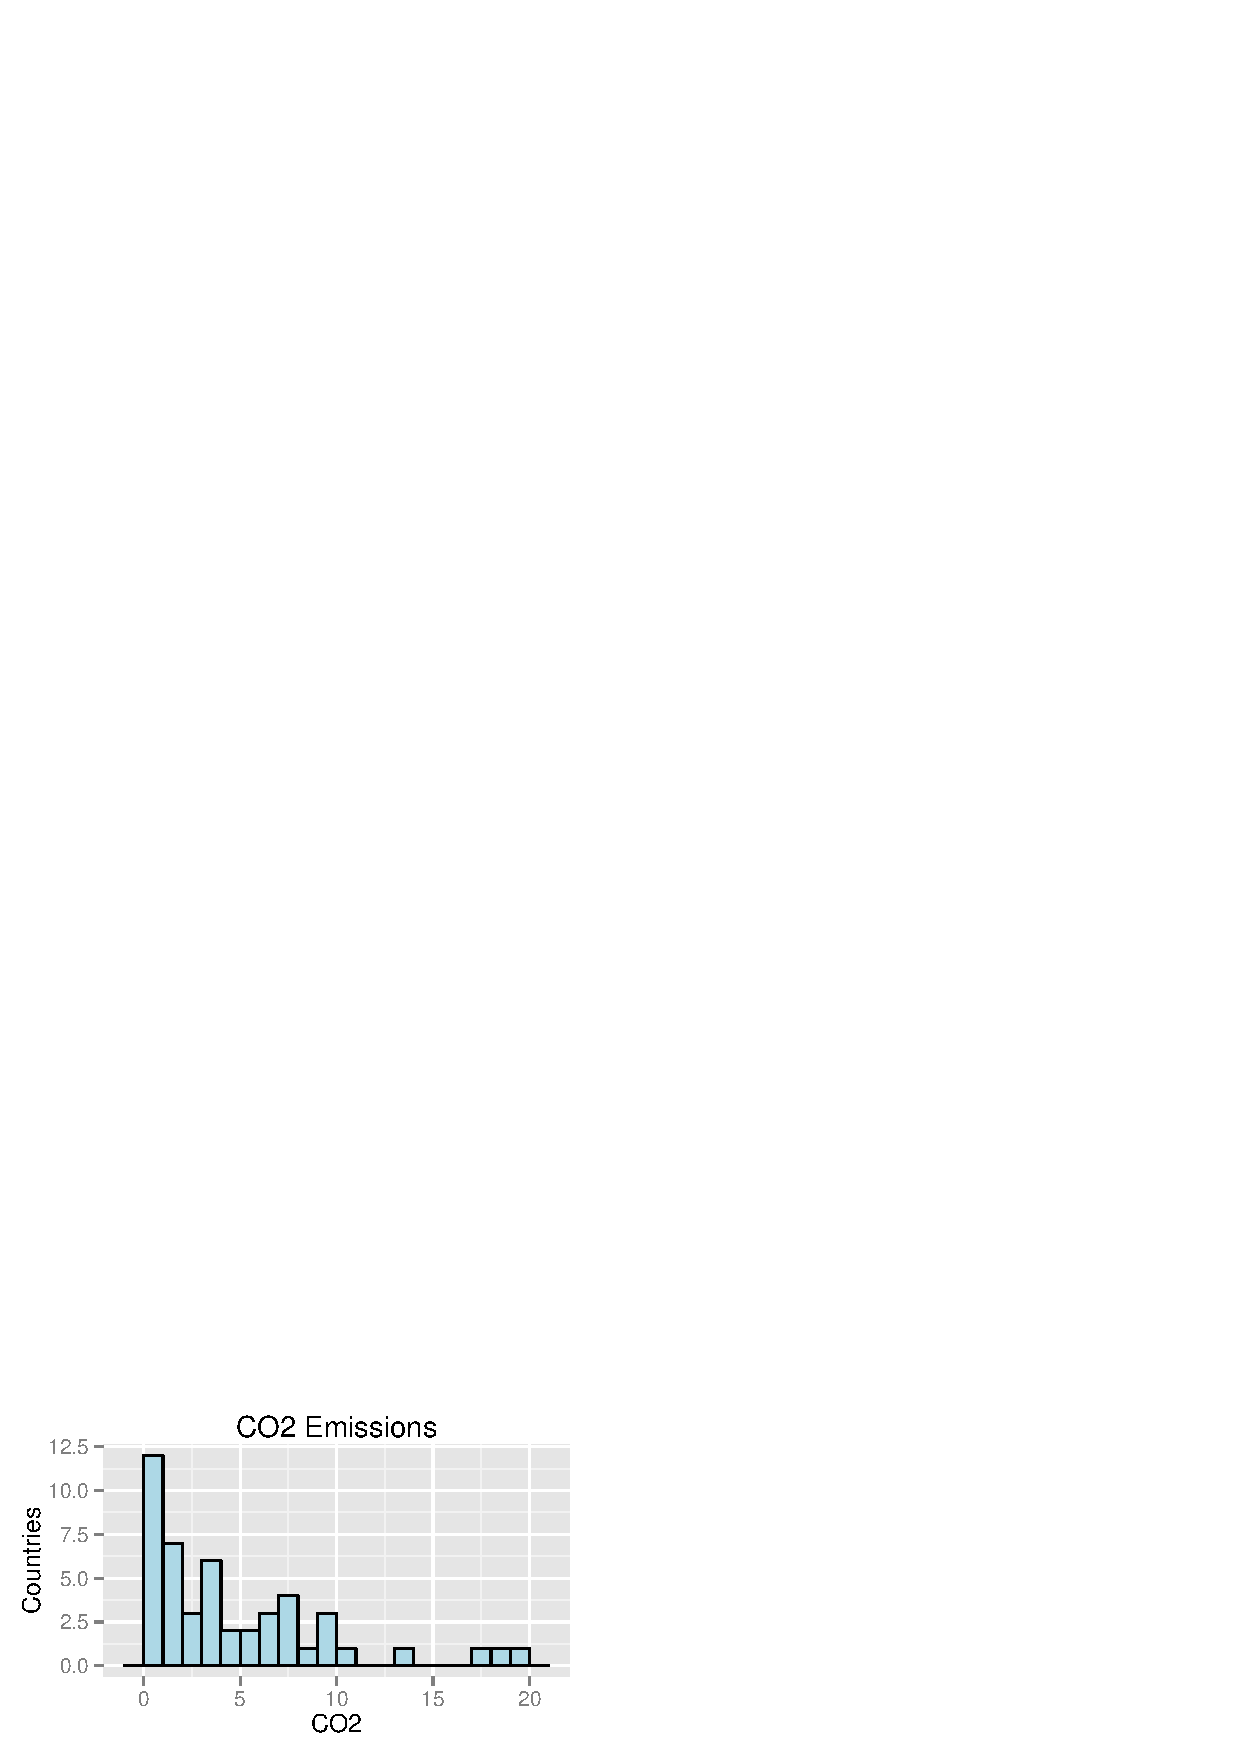
\includegraphics{figures/ex50.pdf}
          \caption{Exercise 50}
        \end{figure}

      \item[51] 
        For a player to be an outlier, he would have to make more than:
        \[
          8,250,000 + (8,250,000 - 425,000) \cdot 1.5 = \$19,987,500
        \]

        None of the players makes this much.

    \end{description}

  \else
    \vspace{11 cm}
    \begin{quote}
      \begin{em}
        All voting is a sort of gaming, like checkers or backgammon, with a
        slight moral tinge to it, a playing with right and wrong, with moral
        questions; and betting naturally accompanies it. 

        % Even voting for the right is doing nothing for it. It is only
        % expressing to men feebly your desire that it should prevail.  A wise
        % man will not leave the right to the mercy of chance, nor wish it to
        % prevail through the power of the majority. There is but little virtue
        % in the action of masses of men. When the majority shall at length vote
        % for the abolition of slavery, it will be because they are indifferent
        % to slavery, or because there is but little slavery left to be abolished
        % by their vote. 
      \end{em}
    \end{quote}
    \hspace{1 cm} --Henry David Thoreau
  \fi

\end{document}

